\label {fs-solution}

\subsection{Reproducibility and Fault Tolerance}

As it was demonstrated in the previous section, {\em exactly once} and determinism are desirable properties for the text classification data flow. On the other hand, one of the key performance metrics in streaming applications is latency, so there is a need to achieve as small latency as possible. Table~\ref{comparison} shows if a system supports exactly once, built-in determinism, and low latency (less than 500 ms). To the best of our knowledge, among open systems only~\FlameStream\ provides for both low latency, determinism, and exactly once. This property is achieved using optimistic order enforcement that implies system-wide idempotence. The details of this approach are discussed in~\cite{we2018adbis, we2018beyondmr}. Therefore, implementation of the text classification data flow on top of~\FlameStream\ can potentially resolve the trade-offs between reliability and performance.

\begin{table}[htbp]
\caption{Support of exactly once, built-in determinism, and low latency (less than 500ms) by stream processing systems}
\begin{threeparttable}
\begin{tabular}{lccc}
System & Exactly-once & Determinism & Latency    \\
\hline
Storm  &    --      &   --       &   low            \\
Heron  &    --      &   --       &   low            \\
Samza  &    --      &   --       &   low            \\
Spark Streaming    &    +       &   +        &   high           \\
Flink              &    +       &   -        &   high$^*$       \\
MillWheel          &    +       &   +        &   NA             \\
FlameStream        &    +       &   +        &   low            \\
\end{tabular}
* with enabled {\em exactly once}~\cite{we2018beyondmr}
\end{threeparttable}
\label{comparison}
\end{table}

\subsection{Concept Drift}

Streaming applications often experience {\em concept drift}: the statistical properties of the target, which the machine learning model is trying to predict, change over time. Regarding news articles classification, concept drift may lead to the following effects:

\begin{itemize}
    \item Meaning of some terms is changing over time. For example, word {\em goal} in the article published during the soccer world cup is most likely related to soccer. On the other hand, during the world hockey cup, it rather belongs to the hockey topic.
    \item News topic may appear and vanish over time. For example, some important events can transform into a separate news topic for a time as it happens with large political or sports forums. However, after some time such topics can disappear form a news agenda.
\end{itemize}

A streaming classifier must handle such behavior in order to automatically fit in rapidly changing news data. We propose a modification of the data flow for prediction with online training that aims to handle concept drift. Training is a separate branch within the logical graph presented in section~\ref{fs-framework}. The modified data flow is shown in Figure~\ref{training_graph}. Assume that the input stream consists of two types of elements: pre-labeled and raw. The latter elements must be labeled by a classifier and delivered to end-user. For already labeled text its features are sent to a {\em Partial fit} vertex instead of the {\em Classifier}. {\em Partial fit} vertex updates machine learning model and sends it to {\em Text Classifier} vertice.

\begin{figure}[htbp]
  \centering
  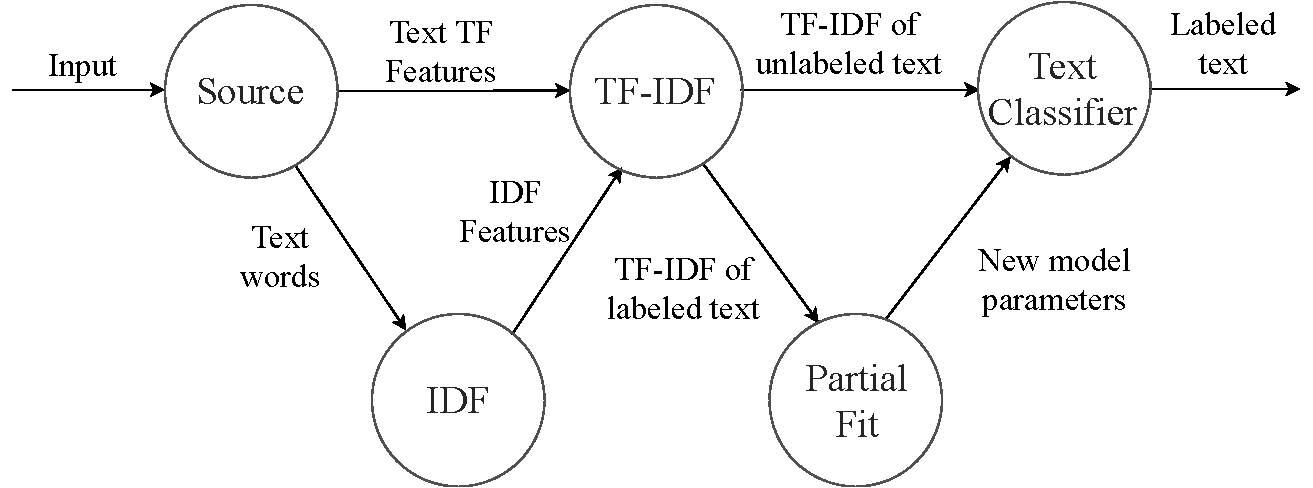
\includegraphics[scale=0.38]{pics/logical-graph}
  \caption{Data flow with online training}
  \label {training_graph}
\end{figure}

A potential issue is that the training process may be time-consuming. If training and prediction processes run consecutively, there will be significant latency spikes, e.g. if a training process lasts for several minutes, then spikes may be thousands times greater than the latency for prediction. However, without synchronization, there will be no reproducible correspondence between texts and applied model. It is almost impossible to achieve the same results within a new run on the same data because the training time becomes a hidden parameter that influences output. 

For instance, assume that we make two runs. On the first run model update takes 70 seconds, but on the second run 75 seconds due to extra CPU load. If training and predicting are not synchronized, more unlabeled input elements are processed by an outdated model in the second case so the distribution of news topics may be different between these two runs. In order to solve this issue, we propose using efficient online learning algorithms, e.g. FTRL proximal~\cite{mcmahan2013ad}. In this case, model updating is smooth and its synchronization with training does not cause latency spikes.